\documentclass{article}
\usepackage[utf8]{inputenc}
\usepackage{graphicx}
\graphicspath{ {./images/} }
\usepackage{amsmath}
\usepackage{hyperref}
%\usepackage[english]{babel}

\usepackage[left=2cm,right=1cm, top=2cm,bottom=2cm,bindingoffset=0cm]{geometry}

\renewcommand{\normalsize}{\fontsize{14}{18pt}\selectfont}

\title{Studying antibiotic resistance via alignment and variants detection}
\author{ Kamilla Faizullina, Ignat Sonets}
\date{\empty}

\begin{document}


\maketitle
In this project, we analyze sequencing data from a strain of E. coli in order to find variants which could lead to the resistance to the antibiotic ampicillin. We use open-source tools to process data and detect mutations. We found the positions of variants in the genome and suggest the possible effects of each mutations. 

\section{Introduction}
Antibiotics are the powerful drugs which used to treat or prevent some types of bacterial infection. However, the enormous and irresponsible use of the antibiotics  has contributed significantly to the advent of the resistant strains \cite{anti}, \cite{anti2}. Development of new antibiotics can be helpful. To that end, scientists carry out researches related to mechanism of resistance. 
\\
In this work, we use the set of real sequencing data from a strain of E.coli resistant to the antibiotic ampicillin in order to analyze it and detect single-nucleotide polymorphism (SNP). The project aims to find the mutated genes to research the mechanism of resistance and attempt to  make recommendations for alternative antibiotics. 
 
\section{Methods}
\subsection{Data}

\begin{table}[h!]
	\centering
	\begin{tabular}{||c c ||} 
		\hline
		Sequencing data  &  Number of reads    \\ [0.5ex] 
		\hline\hline
		Original  & 455876    \\ 
		Improved & 446259 \\ [1ex] 
		\hline
	\end{tabular}
	\caption{Number of reads }
	\label{table:reads}
\end{table}



First, We use the reference  sequence of the  Escherichia coli strain \cite{datalink}. This is E.coli strain K-12 substrain MG1655, laboratory workhorse.  Second, we use the sequencing data of an E. coli strain which is resistant to the antibiotic ampicillin \cite{datalink_res}.

We use Fastqc for the quality control \cite{fqc} (See \ref{sec:supplement}).  With the aim to improve the overall quality of the sequencing data Trimmomatic tool is applied \cite{trim}. We cut off  off the start and the end of a read if quality below 20. We also drop the reads if their lengths are below 20. The window size is 10 and  the average quality  within the window 20. 

 Both forward and reverse initial data consist of 455876 reads. The improved data contains 446259 reads.  \\

\subsection{Aligning sequences to reference}
As we need to map the data from the resistant strain to the reference sequence, we use the aligner called BWA-MEM \cite{bwa}. In order to prepare the data we use \cite{sam}. This utility allows to index and sort bam-format files.

VarScan is used to find SNP \cite{var}. VarScan allows to change the threshold which regulates if  the position is called mutation. We decided to use --min-var-frequency=0.95. 

\section{Results}
First, we improve sequencing data quality of the resistant strain and index data. After, we align the sequence from resistant strain to the reference sequence to detect variants. 
 

The filtered data is used to detect the variants. Five variants is found. 

\begin{table}[h!]
\centering
\begin{tabular}{||c c c  ||} 
 \hline
Position  & Ref & Alt    \\ [0.5ex] 
 \hline\hline
93043 & C & G  \\ 
482698 & T & A    \\
852762 & A & G   \\
3535147 & A & C   \\ 
4390754 & G & T  \\ [1ex] 
 \hline
\end{tabular}
\caption{Results }
\label{table:2}
\end{table}


\section{Discussion}
Position 852762 does not codes protein according to NCNI \cite{ncbi}.

The changing in position 852762 could affect the EG11704 (EcoCyc) which codes multidrug efflux pump RND permease AcrB. This is the inner membrane component of a tripartite.

The variants in position 3535147 could change the gene  EG10269 (EcoCyc). This is the member of the two-component regulatory system EnvZ/OmpR.

Mutation in position 93043 affects the gene G7841 (EcoCyc) which codes small ribosomal subunit biogenesis GTPase RsgA. RsgA induces local conformational changes in the 30S subunit and may thereby destabilize kinetically trapped assembly intermediates

Mutation in position 93043 affects the gene EG10341 (EcoCyc) \cite{ecocyc}. This part of the genome decodes FtsI (penicillin-binding protein 3, PBP3) \cite{uniprot}. Penicillin-binding protein is essential cell division protein that catalyzes cross-linking of the peptidoglycan cell wall at the division septum. The variants of this gene could make strain resistant to antibiotic.


 \section{Supplement}
 \subsection{Improvement of the overall quality of the initial data}
 \label{sec:supplement}
\begin{figure}[h]

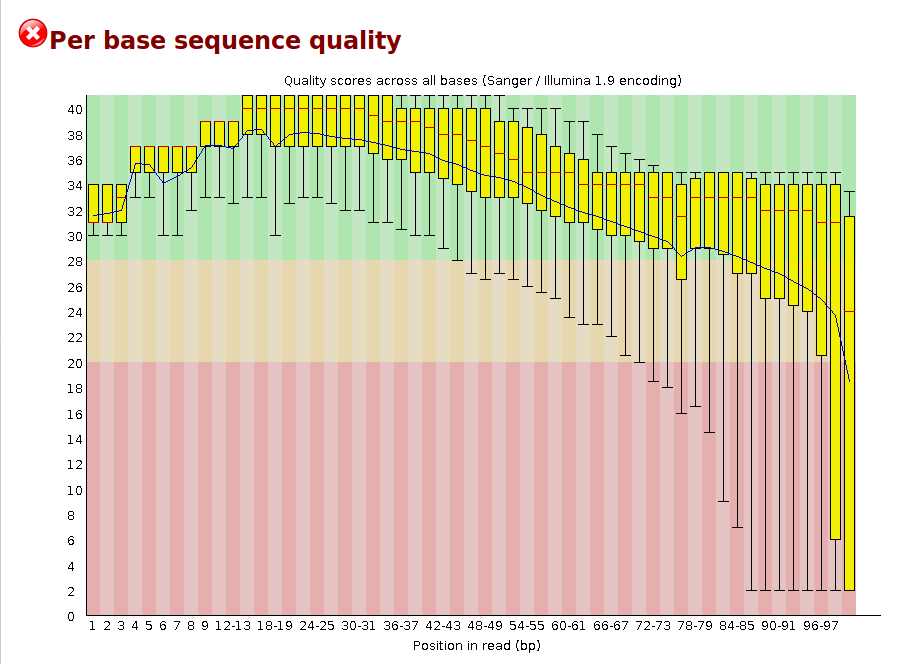
\includegraphics[scale=0.35]{fow_prev_trim.png} 
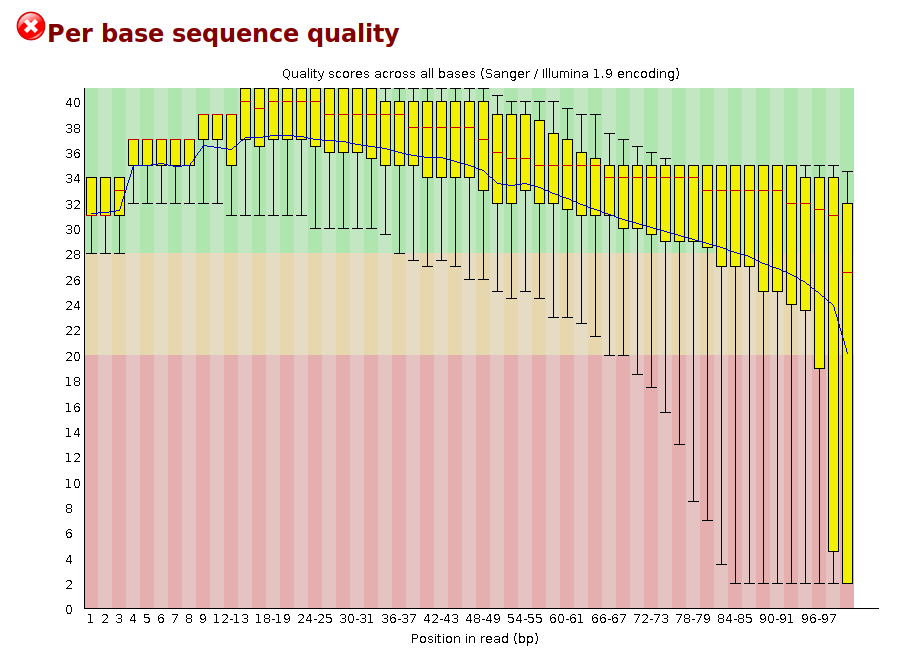
\includegraphics[scale=0.35]{rev_prev_trim.png} \\
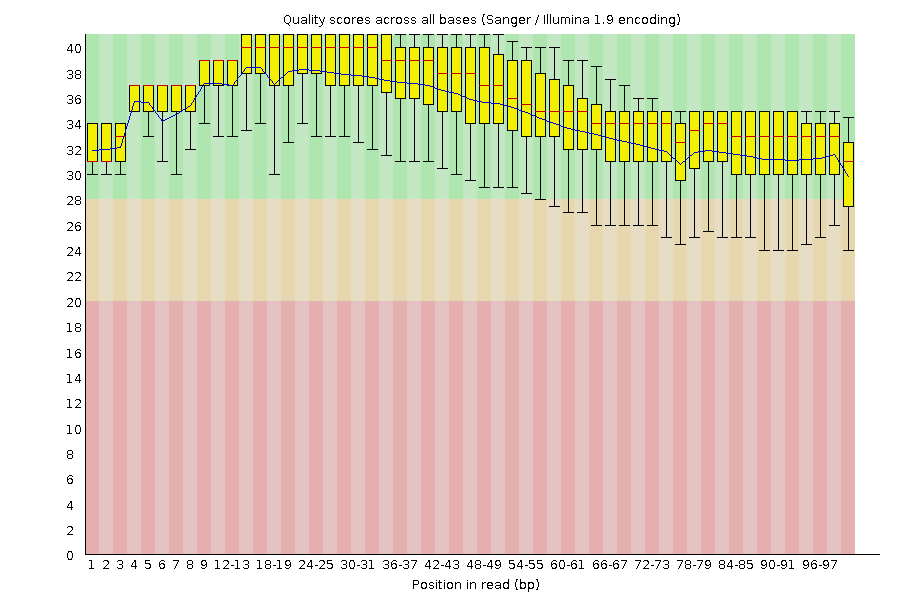
\includegraphics[scale=0.35]{fow_aft_trim.png}
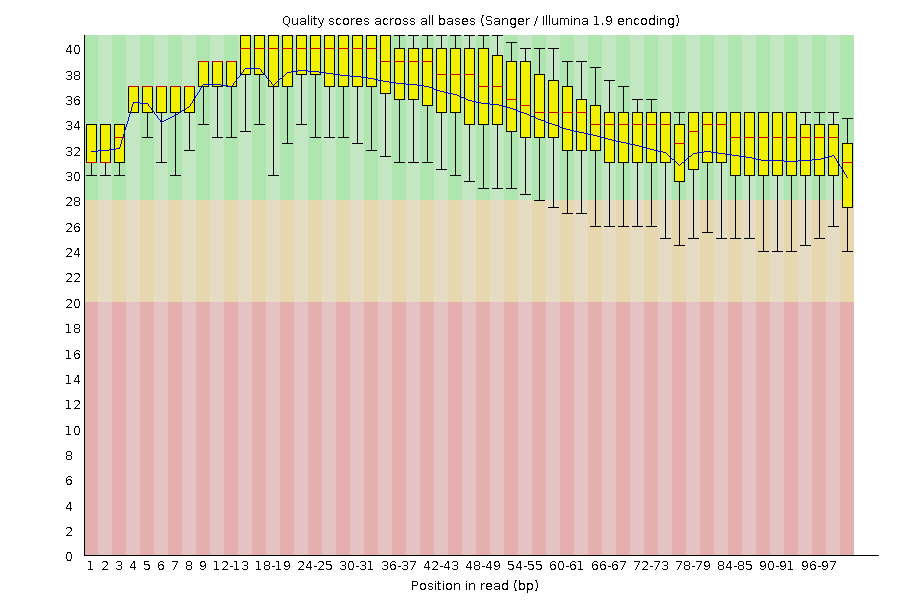
\includegraphics[scale=0.35]{rev_aft_trim.png}
\caption{ The quality of forward (left) and reverse (right) sequence before and after applying Trimmomatic  }
\label{saw}
\end{figure}


\newpage
\begin{thebibliography}{9}

\bibitem{anti} 
Zaman SB, Hussain MA, Nye R, Mehta V, Mamun KT, Hossain N. A Review on Antibiotic Resistance: Alarm Bells are Ringing. Cureus. 2017;9(6):e1403. Published 2017 Jun 28. doi:10.7759/cureus.1403 

\bibitem{anti2}
Ventola CL. The antibiotic resistance crisis: part 1: causes and threats. P T. 2015;40(4):277–283. 

\bibitem{datalink}
The reference data, retrieved  from \href{ftp://ftp.ncbi.nlm.nih.gov/genomes/all/GCA/000/005/845/GCA_000005845.2_ASM584v2}{NCBI FTP}
 
\bibitem{datalink_res}
The data of resistant strains:  \href{http://public.dobzhanskycenter.ru/mrayko/amp_res_1.fastq.zip}{first} and 
\href{http://public.dobzhanskycenter.ru/mrayko/amp_res_2.fastq.zip}{second} 

\bibitem{fqc}
\href{https://www.bioinformatics.babraham.ac.uk/projects/fastqc/}{Fastqc}

\bibitem{trim}
\href{http://www.usadellab.org/cms/?page=trimmomatic}{Trimmomatic: A flexible read trimming tool for Illumina NGS data}

\bibitem{bwa}
\href{http://bio-bwa.sourceforge.net/}{Burrows-Wheeler Aligner}

\bibitem{sam}
\href{http://samtools.sourceforge.net/}{SAM (Sequence Alignment Map) }

\bibitem{var}
\href{http://dkoboldt.github.io/varscan/}{VarScan }
 \bibitem{ncbi}
\href{ https://www.ncbi.nlm.nih.gov/nuccore/NC_000913.3?report=graph}{NCBI }
 
 \bibitem{ecocyc}
\href{https://biocyc.org/gene?orgid=ECOLI&id=EG10341}{EcoCyc }

 \bibitem{uniprot}
\href{https://www.uniprot.org/uniprot/P0AD68}{UniProt}


\end{thebibliography}

\end{document}
